
  
\section{Background}
\label{sec:background}
This section presents the background information for policy-based software systems, XACML policies, regression testing
as well as definitions.

\subsection{Policy-based Software Systems: PEP-PDP separation}
Policy-based software systems are regulated by access control policies that specify the different actions that subjects are allowed to perform on system resources. 
The policy is enforced by one or multiple Policy Enforcement Points (PEP) at the application level. A given PEP receives a subject access request and 
sends it to a Policy decision Point (PDP) that evaluates access control requests against policy rules. The evaluation process involves resolving all the rules in the policy. 
Current access control implementations follow a design strategy that separates between the PEP and the PDP, this separation is advocated mainly for two reasons:
\begin{itemize}
\item Specifying the policy independently from the program enables to save time, cost and effort during the maintenance phase since developers are not required 
to update the application code at each policy update.
\item When the policy is not hard-coded into the application, it can be specified in a standardized language and transported through many different systems platforms.
\end{itemize}
Access control policies can be specified in many languages like EPAL \cite{epal} or XACML \cite {oasis05:xacml}. 
In this paper, we consider XACML polices described in Section~\ref{sec:xacmlpolicies}.


\subsection{XACML Policies} \label{sec:xacmlpolicies}
This section describes the background in the field of XACML policies, policy models, and regression testing.

\begin{figure}[t]
    \centering
        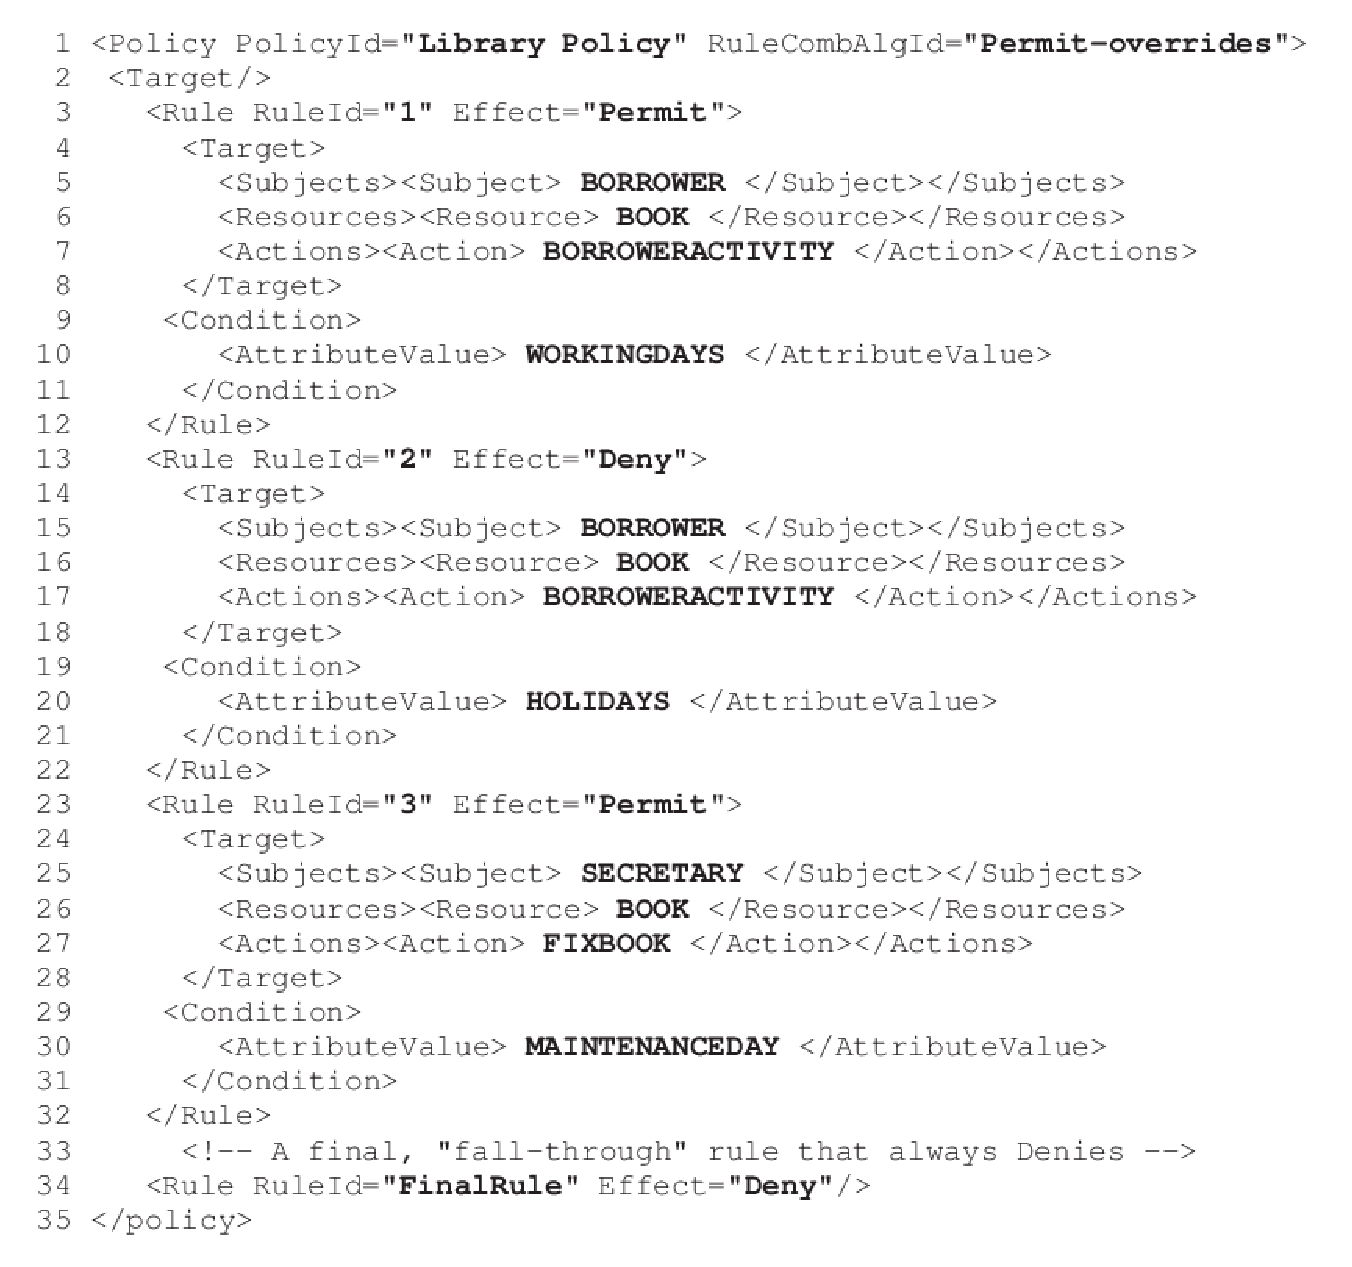
\includegraphics[width=3.7in]{example_policy.eps}
        \vspace{-5pt}
    \caption{\label{fig:example}An example policy specified in XACML}
    \vspace{-10pt}
%    \vspace{+3pt}
\end{figure}
%
%\begin{figure*}[t]%{t}
%%\begin{figure}[firstnumber=100]
%\begin{CodeOut}
%%\tiny % Too samll
%\begin{alltt}
% 
% 1 <Policy PolicyId="\textbf{Library Policy}" RuleCombAlgId="\textbf{Permit-overrides}">
% 2  <Target/>
% 3    <Rule RuleId="\textbf{1}" Effect="\textbf{Permit}">
% 4      <Target>
% 5        <Subjects><Subject> \textbf{BORROWER} </Subject></Subjects>
% 6        <Resources><Resource> \textbf{BOOK} </Resource></Resources>
% 7        <Actions><Action> \textbf{BORROWERACTIVITY} </Action></Actions>
% 8      </Target>
% 9	    <Condition>
%10        <AttributeValue> \textbf{WORKINGDAYS} </AttributeValue>
%11      </Condition>
%12    </Rule>
%13    <Rule RuleId="\textbf{2}" Effect="\textbf{Deny}">
%14      <Target>
%15        <Subjects><Subject> \textbf{BORROWER} </Subject></Subjects>
%16        <Resources><Resource> \textbf{BOOK} </Resource></Resources>
%17        <Actions><Action> \textbf{BORROWERACTIVITY} </Action></Actions>
%18      </Target>
%19	    <Condition>
%20        <AttributeValue> \textbf{HOLIDAYS} </AttributeValue>
%21      </Condition>
%22    </Rule>
%23    <Rule RuleId="\textbf{3}" Effect="\textbf{Permit}">
%24      <Target>
%25        <Subjects><Subject> \textbf{SECRETARY} </Subject></Subjects>
%26        <Resources><Resource> \textbf{BOOK} </Resource></Resources>
%27        <Actions><Action> \textbf{FIXBOOK} </Action></Actions>
%28      </Target>
%29	    <Condition>
%30        <AttributeValue> \textbf{MAINTENANCEDAY} </AttributeValue>
%31      </Condition>
%32    </Rule>
%33      <!-- A final, "fall-through" rule that always Denies -->
%34    <Rule RuleId="\textbf{FinalRule}" Effect="\textbf{Deny}"/>
%35 </policy>
%\end{alltt}
%\end{CodeOut}
%\vspace*{-3.0ex} \caption{An example policy specified in XACML}
% \label{fig:example}
%\end{figure*}

XACML (eXtensible Access Control Markup Language)~\cite{oasis05:xacml} is a language specification standard
%designed by OASIS.
published by the Organization for the Advancement of Structured Information Standards (OASIS).
An XACML access control specification consists of a policy set and a policy combining algorithm.
XACML supports various policy models such as Role Based Access Control (RBAC)~\cite{anderson04:rbacxacml,ferraiolo01:proposed} and Organization-Based Access 
Control (OrBAC)~\cite{kalam03:orBac}. For RBAC and OrBAC, various job functions are associated to roles (e.g., staff or employee) that a user possesses. 
Permissions or denials to take an action on certain objects are assigned to specific roles (instead of users). OrBAC supports 
extra features such as role, activity (i.e., action), and view (i.e., object) hierarchy.
Figure~\ref{fig:example} is an OrBAC policy example where 
roles such as ``Secretary'' and ``Borrower'' are associated with subject attributes and policy decisions are made through 
specific roles.

Let $Conditions$ be the set of the environmental context
such as working days or holidays, a file size, and a user's task authorization level. 
Let $S$, $O$, $A$, and $C$ denote all the subjects,
objects, actions, and  $Conditions$, respectively, in an access control system.

An XACML policy consists of a \Intro{policy set}, which consists
of \Intro{policy sets} and \Intro{policies}. A \Intro{policy} consists
of a sequence of \Intro{rules}, each of which
specifies under what conditions $C$ subject $S$ is allowed or denied
to perform action $A$ (e.g., read) on certain object (i.e., resources) $O$ in a system.

A rule $R$ is of the following form:
\begin{center}
$R$ $\subseteq$ $S$ $\times$ $A$ $\times$ $O$ $\times$ $C$ $\longrightarrow$ $Dec$
\end{center}
where $Dec$ denotes a decision, which is either permit or deny.
A user's request is evaluated against a policy.
A request matches with a rule if the request satisfies the rule's
attributes. Then the rule's decision can be returned.
Formally, a request $Q$ in the following form matches $R$:
\begin{center}
$Q$ $\subseteq$ $S_q$ $\times$ $A_q$ $\times$ $O_q$ $\times$ $C_q$ where $S_q$ $\subseteq$ $S$, $A_q$ $\subseteq$ $A$, $O_q$ $\subseteq$ $O$, and $C_q$ $\subseteq$ $C$.
\end{center}


More than one rule in a policy may be applicable to a given request.
The \Intro{rule combining algorithm} is used to combine multiple
rule decisions into a single decision. There are four standard rule
combining algorithms: \CodeIn{deny-overrides}, \CodeIn{permit-overrides}, \CodeIn{first
applicable}, and \CodeIn{only-one-applicable}. The
\Intro{deny-overrides algorithm} returns \CodeIn{Deny} if any rule
evaluation returns \CodeIn{Deny} or no rule is applicable. The
\Intro{permit-overrides algorithm} returns \CodeIn{Permit} if any
rule evaluation returns \CodeIn{Permit}. Otherwise, the algorithm
returns \CodeIn{Deny}.
The \Intro{first-applicable algorithm} returns whatever the
evaluation of the first applicable rule returns. The
\Intro{only-one-applicable} algorithm returns the decision of the only
applicable rule if there is only one applicable rule, and returns
error otherwise.

Figure~\ref{fig:example} shows a policy specified
in XACML. The policy consists of three XACML rules used in our real-life library access
control policy subject, called $LMS$~\cite{mouelhi09:tranforming}.
Note that we simplified XML formats to reduce
space for this example.
Lines 3-12 describe a rule that \CodeIn{borrower} is permitted to \CodeIn{borroweractivity} (e.g., borrowing books) \CodeIn{book} in \CodeIn{working days}.
Lines 13-22 describe a rule that \CodeIn{borrower} is denied to \CodeIn{borroweractivity} \CodeIn{book} in \CodeIn{holidays}.
Lines 23-32 describe a rule that \CodeIn{secretary} is permitted to \CodeIn{fixing} for \CodeIn{book} in \CodeIn{maintenance day}.
As these rules are combined using the permit-overrides algorithm, the \Intro{permit-overrides algorithm} returns the \CodeIn{Permit} if
 a request matches at least one of rules with permit decisions. For example, if rules 2 and 3 are applicable to a request, the decision
evaluated from rule 3 is given higher priority than that of rule 2.


\subsection{Regression Testing}
Software testing \cite{Myers:1979:AST:539883} refers to the activity of generating Tests Cases to verify the conformity of output results provided by a 
program to the expected output that meets its functional and non functional requirements. With the increasing complexity of software systems, 
this activity is gaining more and more interest in the research field and aiming to establish a trade-off between cost, time and quality. 
%%%%link%%%%

Software is subject to changes that occur at the design stage or in later stages at the deployment or maintenance phases. These changes are 
usually supposed to meet changes in the requirements or to overcome errors that can be detected in later stages of software life cycle. 
Regression testing refers to the research field that is interested in retesting the system to verify that the new changes have not altered 
the initial system behavior. As highlighted by Rothermel et al. in \cite{Rothermel:1996:ART:235681.235682}, regression testing is defined like the 
following: 
``Given a program $P$, a modified version $P'$, and a set $T$ of test cases used previously to test $P$, regression analysis and testing 
techniques attempt to make use of a subset of $T$ to gain sufficient confidence in the correctness of $P'$ with respect to behaviors from $P$ retained 
in $P'$''.

The main objectives of regression testing is to reduce the cost of rerunning initial test cases and to maximize the capability of 
selected test cases to detect potential faults induced by changes.
To the best of our knowledge, there is no previous research work on regression testing that considers policy changes in policy-based software systems. 
The global scenario that illustrates regression testing process for such systems is presented in Figure~\ref{fig:process}.
In the scenario, our test-selection technique identifies the changed policy behaviors (
i.e., rules impacted by policy changes)
 between a policy $P$ and its modified version $P'$ and selects only the portion of test cases $T'$ to reveal different behaviors
impacted by policy changes. If there exists the changed policy behaviors not-covered with $T'$, our test augmentation technique generates additional test cases $T''$  to achieve 100\% coverage of the changed policy behaviors.
%In the next section, we present our three test selection techniques and our test augmentation technique.

In this paper, we classify system test cases into two types illustrated in Figure~\ref{fig:systemtestcases}.
The first one is a set of functional system test cases, which
are produced based on functional requirements, but do not involve
in testing security requirements such as triggering application code to generate
and evaluate requests against a policy under test.
The second one is a set of security system test cases, which
involve in triggering application code to generate
and evaluate requests against a policy under test.
Security system test cases may include test oracles
to determine whether program behaviors interacting with a policy
are correct.


%\FixJeeHyun{The figure \ref {} illustrates the overall scenario of regression testing applied to policy-based software systems\\
%ADD schema}
%
%
\begin{figure}[t]
    \centering
        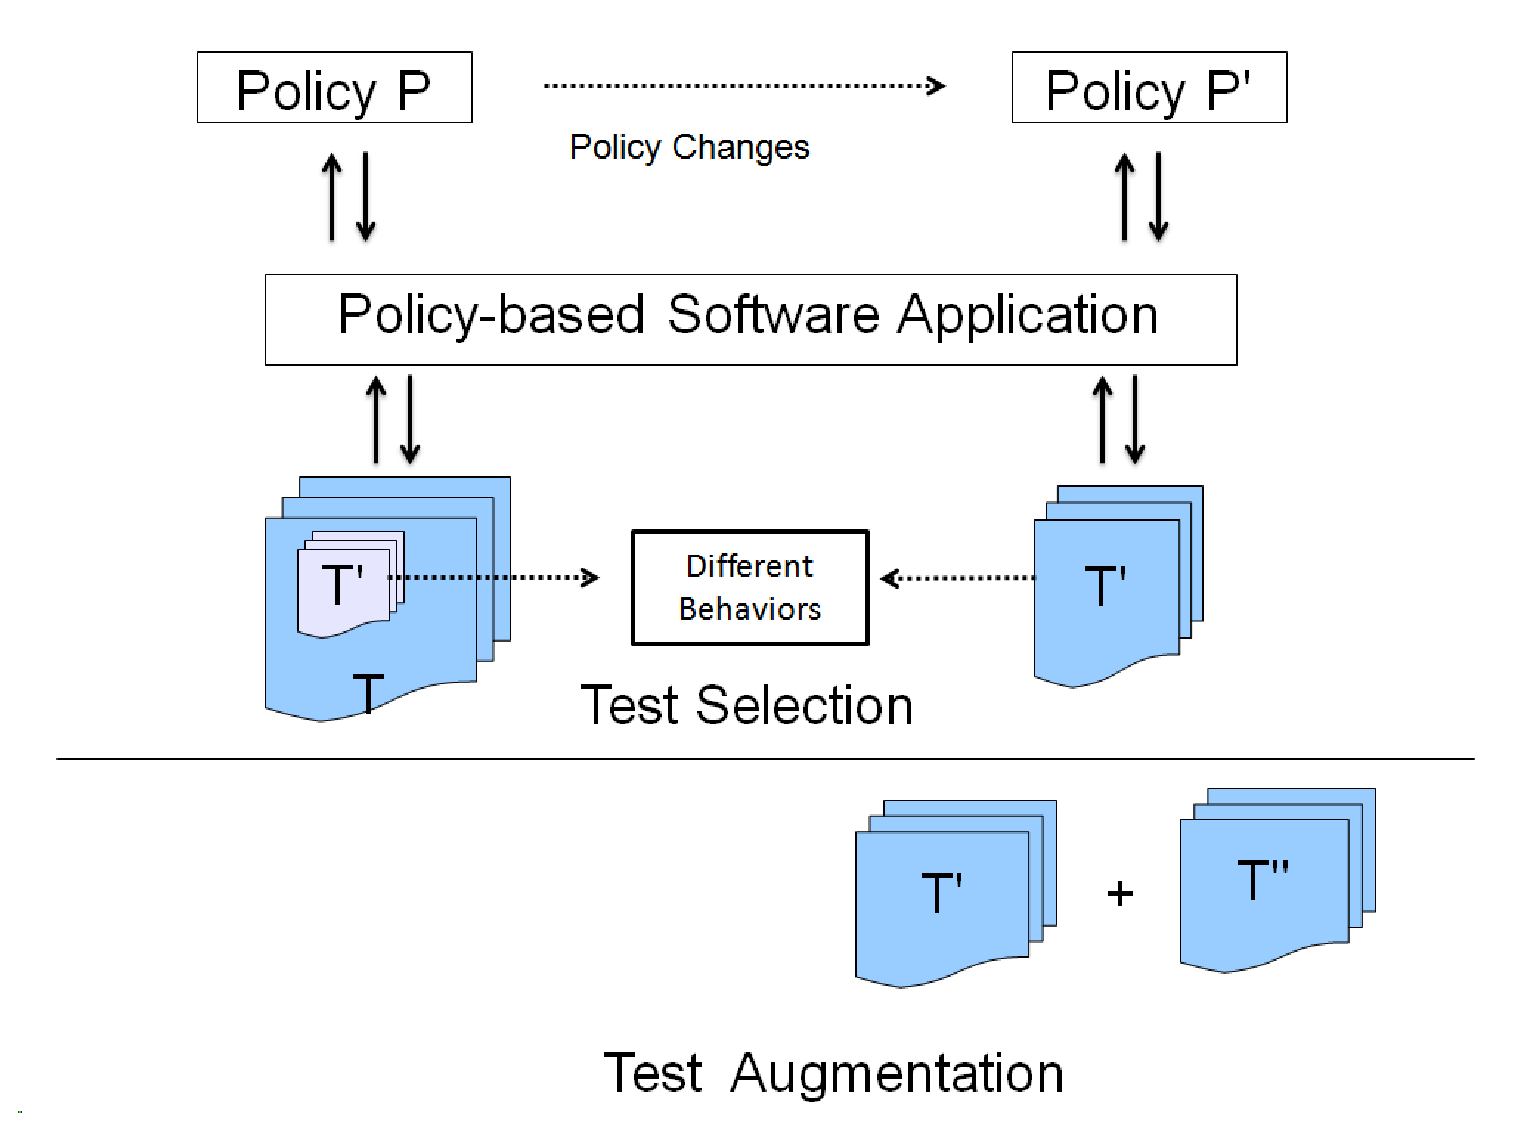
\includegraphics[width=3.5in]{regressiontesting.eps}
       \vspace{-4pt}
    \caption{\label{fig:process}Regression Testing Process}
   \vspace{-10pt}
%    \vspace{+3pt}
\end{figure}
\begin{figure}[t]
    \centering
    \vspace{+5pt}
        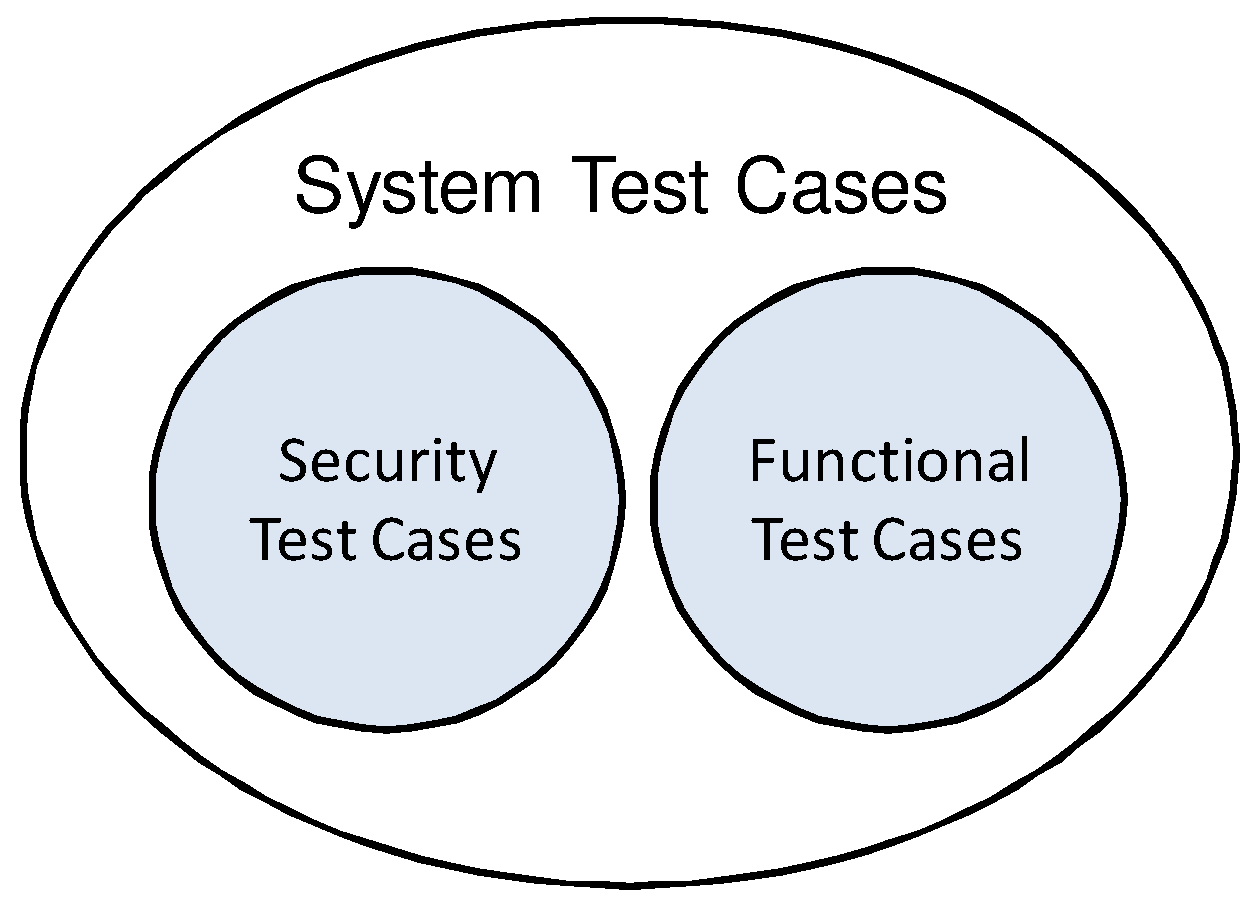
\includegraphics[width=2.5in]{systemtestcases.eps}
       \vspace{-4pt}
    \caption{\label{fig:systemtestcases}System test cases}
   \vspace{-10pt}
    \vspace{+3pt}
\end{figure}

%\subsection{Definitions}
%
%Security policy testing (SP testing): it denotes the activity
%of generating and executing test cases that
%are derived specifically from a SP. The objective of
%SP testing is to reveal as many security flaws as
%possible.
%Test case: In the paper, we define a test case as a triplet:
%intent, input test sequence, oracle function.
%
%To help answer these questions, we collect several metrics to
%to show effectiveness and efficiency of our test selection techniques and
%our test augmentation technique. 
%The following metrics are
%measured for each subject under test interacting with each modified policy
%and each technique.
%\begin{itemize}
%%	\item \textit{Selected test case count}.  The test count is the size of the request set or
%%the number of tests generated by the chosen test-generation
%%technique. For testing access control policies, a test is synonymous with request
%	\item \textit{Functional system test cases.} 
%	The test cases exercise functional requirements of a software system.
%	By opposition with security system test cases, we call these test cases
%	
%	System/functional testing . the activity which consists
%of generating and executing test cases which are
%produced based on the uses cases and the business
%models (e.g. analysis class diagram and dynamic
%views) of the system. By opposition with security
%tests, we call these tests functional.
%
%
%	 Given a policy and its modified
%	policy, the test reduction percentage is the number of selected test cases for regression testing divided by number of security test cases.
%		\item \textit{Modified policy behavior count.}  Given a policy and its modified
%	policy, the modified policy behavior count is the number of impacted rules by policy changes.
%	\item \textit{Modified policy behavior coverage count.}  Given a policy and its modified
%	policy, the modified policy behavior coverage count is the number of
%	impacted rules covered with existing test cases.
%	\item \textit{Modified policy coverage percentage.}  Given a policy and its modified
%	policy, the modified policy behavior coverage percentage is the modified policy behavior coverage count divided the total number of impacted rules.
%	\item \textit{Elapsed time.}  The elapsed time is time (measured in milliseconds) elapsed for each step during the test selection process.
%	\item \textit{Augmented test case count.}  The augmented test case count is the number of augmented test cases by each augmentation type.
%	
%\end{itemize}



